\documentclass[12pt,a4paper]{article}

\usepackage[margin=2.5cm]{geometry}
\usepackage{booktabs}
\usepackage{tabularx}
\usepackage{array}
\usepackage{hyperref}
\usepackage{enumitem}
\usepackage{fancyhdr}
\usepackage{parskip}
\usepackage{titlesec}
\usepackage{xcolor}
\usepackage{graphicx}
\usepackage{float}
\usepackage{mdframed}

\definecolor{accent}{RGB}{30,80,160}
\definecolor{patternbox}{RGB}{240,245,255}

\hypersetup{colorlinks=true, linkcolor=accent, urlcolor=accent}

\titleformat{\section}{\large\bfseries\color{accent}}{}{0em}{}[\titlerule]
\titleformat{\subsection}{\normalsize\bfseries\color{accent}}{}{0em}{}
\titleformat{\subsubsection}{\normalsize\bfseries}{}{0em}{}

\pagestyle{fancy}
\fancyhf{}
\lhead{\textbf{WanderSync} \textit{Task 3: Implementation Patterns}}
\rhead{Team 15}
\rfoot{\thepage}
\renewcommand{\headrulewidth}{0.4pt}

\newcommand{\patternfield}[2]{%
  \noindent\textbf{#1:}\hspace{0.5em}#2\par\vspace{0.3em}%
}

\begin{document}

\begin{center}
  {\LARGE\bfseries Task 3: Implementation Patterns}\\[0.4em]
  {\large WanderSync: Dynamic Itinerary, Disruption Management and Social Travel Hub}\\[0.2em]
  {\normalsize Team 15}
\end{center}

\vspace{1em}

% ================================================================
\section{Overview}
% ================================================================

Two design patterns are applied in WanderSync to address recurring structural problems that
cannot be resolved by architectural tactics alone. Each pattern is documented with its category,
the specific problem it solves within the system, the classes and modules involved, and UML
diagrams showing the structure and runtime behaviour.

% ================================================================
\section{Pattern 1: Observer}
% ================================================================

\begin{mdframed}[backgroundcolor=patternbox, linecolor=accent, linewidth=0.8pt]
\patternfield{Category}{Behavioral}
\patternfield{NFRs addressed}{NFR2 (Reliability -- disruption notification within 10 s); NFR5 (Modifiability -- adding a new reaction type requires no changes to the detection service)}
\end{mdframed}

\vspace{0.5em}

\subsubsection{Problem}

When the Disruption Detection Service identifies a flight delay or cancellation, multiple
independent subsystems must react: the Notification Service must alert the user, the Itinerary
Management Service must flag affected segments, and the Social Synchronisation Service may need
to notify a travel companion. Without a formal decoupling mechanism, the Disruption Detection
Service would hold direct references to all three consumers, creating tight coupling. Every new
reaction type (e.g., a future re-booking suggestion engine) would require modifying the detection
service itself, violating the Modifiability NFR and GRASP Low Coupling.

\subsubsection{Solution and Class Mapping}

The Observer (Publish-Subscribe) pattern decouples the event source from its consumers.

\begin{itemize}[noitemsep]
  \item \textbf{\texttt{DisruptionEvent}} -- data object carrying \texttt{flightId},
        \texttt{DisruptionType}, and \texttt{Instant} timestamp.
  \item \textbf{\texttt{IDisruptionObserver}} -- interface declaring
        \texttt{onDisruption(event: DisruptionEvent)}. All consumers implement this interface.
  \item \textbf{\texttt{DisruptionEventPublisher}} -- subject; holds a list of registered
        \texttt{IDisruptionObserver} instances; calls \texttt{notifyObservers(event)} after
        persisting the event to the Redis Stream (Tactic 4).
  \item \textbf{\texttt{NotificationObserver}} -- sends an in-app or email notification to
        the affected user.
  \item \textbf{\texttt{ItineraryFlagObserver}} -- marks the affected \texttt{BookingRecord}
        segments as disrupted and invalidates the itinerary cache entry.
  \item \textbf{\texttt{SocialAlertObserver}} -- queries the consent registry and notifies
        matched travel companions who have bilateral opt-in with the affected user.
\end{itemize}

Adding a new observer (e.g., a re-booking engine) requires implementing
\texttt{IDisruptionObserver} and registering it at startup -- zero changes to
\texttt{DisruptionEventPublisher}.

\subsubsection{Class Diagram}

\begin{figure}[H]
  \centering
  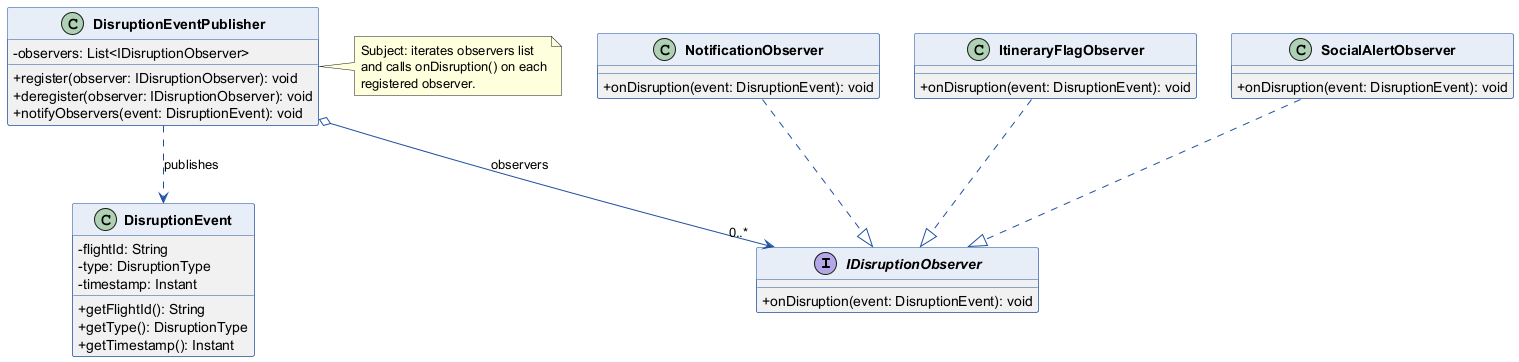
\includegraphics[width=0.9\textwidth]{diagrams/task3_observer.png}
  \caption{Observer Pattern -- Disruption Event Publication}
\end{figure}

% ================================================================
\section{Pattern 2: Chain of Responsibility}
% ================================================================

\begin{mdframed}[backgroundcolor=patternbox, linecolor=accent, linewidth=0.8pt]
\patternfield{Category}{Behavioral}
\patternfield{NFRs addressed}{NFR3 (Security -- 100\% of endpoints require JWT enforcement, HTTPS); NFR5 (Modifiability -- handlers are independently testable and reorderable)}
\end{mdframed}

\vspace{0.5em}

\subsubsection{Problem}

Every inbound request to the API Gateway must pass through multiple independent validation steps
in a defined order: rate-limit check, JWT authentication, request schema validation, and audit
logging. Encoding all these steps as a flat conditional block in a single gateway controller
method produces a God Method that violates High Cohesion (GRASP) and makes each step
impossible to test in isolation. Furthermore, steps must be reorderable (e.g., placing the
audit logger after auth so that only authenticated requests are logged) and individually
enable/disable-able in test environments.

\subsubsection{Solution and Class Mapping}

The Chain of Responsibility pattern organises each processing step as an independent handler
that either processes the request and passes it to the next handler or short-circuits with an
error response.

\begin{itemize}[noitemsep]
  \item \textbf{\texttt{RequestHandler}} -- abstract base class declaring
        \texttt{setNext(handler)}, the protected \texttt{next} reference, and the abstract
        \texttt{handle(request: ApiRequest): ApiResponse} method.
  \item \textbf{\texttt{RateLimitHandler}} -- checks the caller's request count against a
        Redis counter; returns \texttt{429 Too Many Requests} if exceeded.
  \item \textbf{\texttt{AuthHandler}} -- validates the JWT signature and 24-hour expiry;
        returns \texttt{401 Unauthorized} if invalid, satisfying NFR3.
  \item \textbf{\texttt{SchemaValidationHandler}} -- validates the request body against the
        declared schema; returns \texttt{400 Bad Request} on violation.
  \item \textbf{\texttt{AuditLogHandler}} -- writes request metadata (user ID, endpoint,
        timestamp) to the audit log; always passes through to the next handler.
  \item \textbf{\texttt{GatewayController}} -- assembles the chain at startup:
        \texttt{RateLimitHandler $\to$ AuthHandler $\to$ SchemaValidationHandler $\to$
        AuditLogHandler $\to$ route dispatch}. Only this class changes when the chain order
        is modified.
\end{itemize}

\subsubsection{Class Diagram}

\begin{figure}[H]
  \centering
  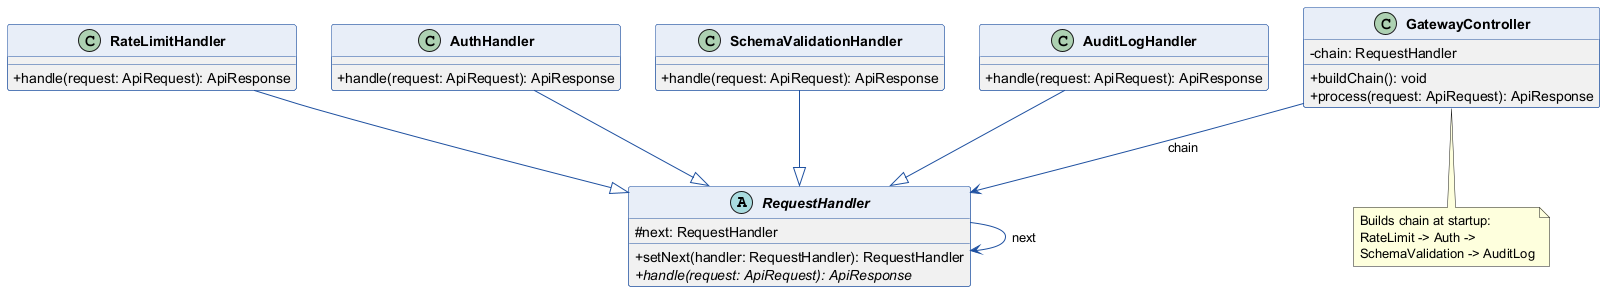
\includegraphics[width=0.82\textwidth]{diagrams/task3_cor_class.png}
  \caption{Chain of Responsibility -- API Gateway Handler Hierarchy}
\end{figure}

\subsubsection{Sequence Diagram}

The sequence diagram below shows a successful request traversing the full chain (happy path)
and a short-circuit at \texttt{AuthHandler} for an invalid JWT (alternate path).

\begin{figure}[H]
  \centering
  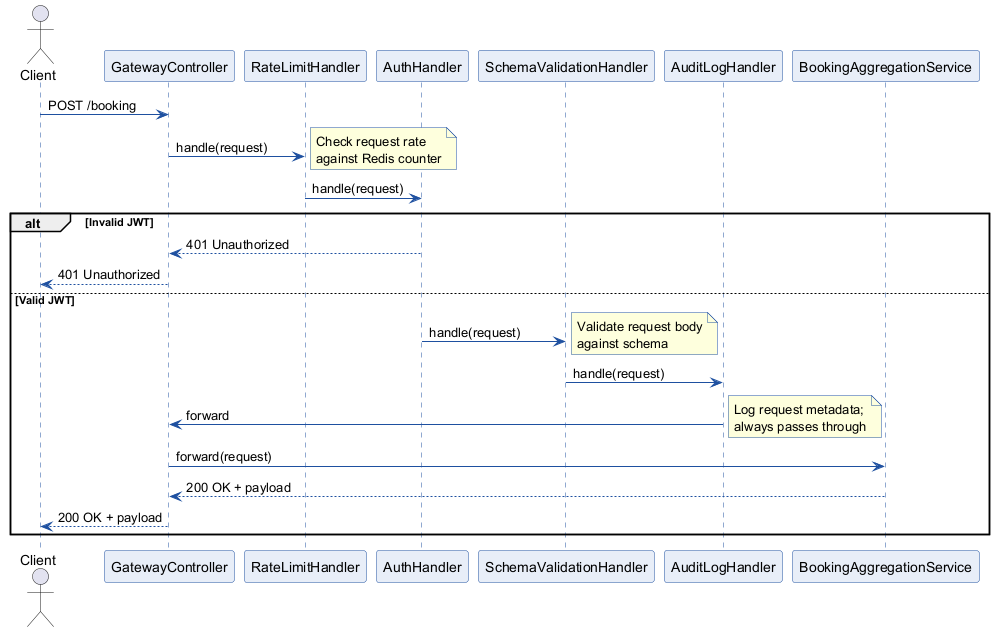
\includegraphics[width=0.9\textwidth]{diagrams/task3_cor_sequence.png}
  \caption{Chain of Responsibility -- Request Handling Sequence (happy path and JWT rejection)}
\end{figure}

% ================================================================
\section{Pattern Summary}
% ================================================================

\begin{tabularx}{\textwidth}{lllX}
\toprule
\textbf{Pattern} & \textbf{Category} & \textbf{NFRs} & \textbf{Key Classes} \\
\midrule
Observer & Behavioral & NFR2, NFR5 &
  \texttt{DisruptionEventPublisher}, \texttt{IDisruptionObserver},
  \texttt{NotificationObserver}, \texttt{ItineraryFlagObserver},
  \texttt{SocialAlertObserver} \\[0.4em]
Chain of Responsibility & Behavioral & NFR3, NFR5 &
  \texttt{RequestHandler}, \texttt{RateLimitHandler}, \texttt{AuthHandler},
  \texttt{SchemaValidationHandler}, \texttt{AuditLogHandler},
  \texttt{GatewayController} \\
\bottomrule
\end{tabularx}

\end{document}
